\cite{ferrand_fluid_2021} ont aussi utilisé des simulations du modèle \sacro{LFHPe} prenant en compte un flux de chaleur $\overline{\overline{\boldsymbol{q}}}$ gyrotrope obtenu grâce à une fermeture Landau-fluide présente dans le code versatile présenté dans la section \ref{sec-311}. Il s'est avéré que ces simulations prennent aussi en compte un tenseur de pression électronique de type gyrotrope.
La fermeture Landau-fluide corrigeant les critères d'instabilité tel que le critère miroir afin de refléter le comportement linéaire cinétique, elle pourrait par la suite nous aider à étendre nos interprétations vers les processus cinétiques. 

Dans ce chapitre, nous décrivons les spécificités du modèle implémenté et la loi exacte complète associée. Une première application préliminaire sur deux simulations semble montrer des résultats paradoxaux qui nécessiteront une étude plus fine avant d'en extraire un début d'interprétation. 


\section{Modèle simulé et loi exacte}
\label{sec-341}

Dans ce deuxième lot de simulations, les ions et les électrons sont décrits avec un tenseur de pression gyrotrope. La fermeture utilisée est une fermeture Landau-fluide. Cette fermeture nous rapproche du comportement cinétique en prenant en compte l'amortissement Landau linéaire (phénomène cinétique) dans le modèle fluide. Cette correction étant basée sur la relation de dispersion cinétique, les critères d'instabilité seront aussi corrigés pour correspondre aux critères cinétiques. La gyrotropie des électrons impactera d'ailleurs le critère miroir. Les flux de chaleur ioniques et électroniques sont aussi supposés gyrotropes.

Les premières équations normalisées du modèle simulé sont, en y faisant apparaître indépendamment les tenseurs des pressions ionique et électronique, : 
\begin{eqnarray}
\label{eq:mlf_r} \partial_t \rho + \nabla \cdot \left(\rho \boldsymbol{v}\right) &=& 0,\\
\label{eq:mlf_v} \partial_t  \boldsymbol{v} + \boldsymbol{v} \cdot \nabla  \boldsymbol{v} - \frac{1}{\rho} \boldsymbol{j} \times \boldsymbol{B} + \frac{1}{\rho} \nabla \cdot \left(\overline{\boldsymbol{P_i}} + \overline{\boldsymbol{P_e}} \right)  &=& 0,  \\
\label{eq:mlf_b} \partial_t \boldsymbol{B} - \nabla \times \left( \boldsymbol{v} \times \boldsymbol{B} \right) +  d_i  \nabla \times \left( \frac{1}{\rho} \boldsymbol{j}\times \boldsymbol{B} \right) &=& d_i \nabla \times \left( \frac{1}{\rho} \nabla \left(  p_e\right) \right),
\end{eqnarray}
\begin{eqnarray}
\label{eq:mlf_pperpi} \partial_t  p_{\perp i }  +  \nabla \cdot \left(p_{\perp i } \boldsymbol{v} \right) +  p_{\perp i }\nabla \cdot\boldsymbol{v} -  p_{\perp i } \boldsymbol{b}\boldsymbol{b} : \nabla \boldsymbol{v}  &=& - \frac{1}{2} \left( \text{Tr}(\nabla \cdot \overline{\overline{\boldsymbol{q_i}}}) - \boldsymbol{b}\boldsymbol{b} : \nabla \cdot \overline{\overline{\boldsymbol{q_i}}} \right), \nonumber \\ && \\
\label{eq:mlf_ppari} \partial_t  p_{\parallel i }  +  \nabla \cdot \left(p_{\parallel i } \boldsymbol{v} \right) +  2 p_{\parallel i }  \boldsymbol{b}\boldsymbol{b} : \nabla \boldsymbol{v}  &=&  - \boldsymbol{b}\boldsymbol{b} : \nabla \cdot \overline{\overline{\boldsymbol{q_i}}},   \\
\label{eq:mlf_pperpe} \partial_t  p_{\perp e }  +  \nabla \cdot \left(p_{\perp e } \boldsymbol{v_e} \right) +  p_{\perp e }\nabla \cdot\boldsymbol{v_e} -  p_{\perp e } \boldsymbol{b}\boldsymbol{b} : \nabla \boldsymbol{v_e}  &=&  - \frac{1}{2} \left( \text{Tr}(\nabla \cdot \overline{\overline{\boldsymbol{q_e}}}) - \boldsymbol{b}\boldsymbol{b} : \nabla \cdot \overline{\overline{\boldsymbol{q_e}}} \right), \nonumber \\ && \\
\label{eq:mlf_ppare} \partial_t  p_{\parallel e }  +  \nabla \cdot \left(p_{\parallel e } \boldsymbol{v_e} \right) +  2 p_{\parallel e }  \boldsymbol{b}\boldsymbol{b} : \nabla \boldsymbol{v_e}  &=& - \boldsymbol{b}\boldsymbol{b} : \nabla \cdot \overline{\overline{\boldsymbol{q_e}}}, 
\end{eqnarray}
avec $\overline{\boldsymbol{P_{i,e}}} =  \frac{\beta_0}{2} \left(p_{\perp i,e } \overline{\boldsymbol{I}} + \left(p_{\parallel i,e } - p_{\perp i,e }\right) \boldsymbol{b} \boldsymbol{b} \right) $ les tenseurs gyrotropes des pressions ionique (i) et électronique (e), $\boldsymbol{b} = \frac{\boldsymbol{B}}{|\boldsymbol{B}|}$ la direction du champ magnétique, $\frac{\beta_0}{2} $ la constante provenant de la normalisation des équations, et $\boldsymbol{v_e} = \boldsymbol{v} - d_i \frac{\boldsymbol{j}}{\rho} $ la vitesse électronique. La fermeture est appliquée au niveau du quatrième moment\footnote{Pour plus d'informations, se référer aux premières parties de \cite{passot_collisionless_2007}.} présent dans les équations de $ \overline{\overline{\boldsymbol{q_i}}}$ et $ \overline{\overline{\boldsymbol{q_e}}}$. L'hypothèse de gyrotropie appliquée aux tenseurs de flux de chaleur implique (avec $s = i,e$) :  
\begin{eqnarray*}
    \boldsymbol{b}\boldsymbol{b} : \nabla \cdot \overline{\overline{\boldsymbol{q_s}}} &\simeq& \nabla \cdot (q_{\parallel s} \boldsymbol{b}) - 2 q_{\perp s} \nabla \cdot \boldsymbol{b},\\
    \frac{1}{2} \left( \text{Tr}(\nabla \cdot \overline{\overline{\boldsymbol{q_s}}}) - \boldsymbol{b}\boldsymbol{b} : \nabla \cdot \overline{\overline{\boldsymbol{q_s}}} \right)  &\simeq&  \nabla \cdot (q_{\perp s} \boldsymbol{b})  + q_{\perp s} \nabla \cdot \boldsymbol{b}.
\end{eqnarray*}


L'équation d'énergie interne peut être construite à partir des équations des pressions \eqref{eq:mlf_ppari}, \eqref{eq:mlf_pperpi}, \eqref{eq:mlf_ppare}, \eqref{eq:mlf_pperpe} et de la relation $\boldsymbol{v_e} = \boldsymbol{v} - d_i \frac{\boldsymbol{j}}{\rho} $. Ainsi, on obtient :
\begin{eqnarray}
\label{eq:mlf_ui} \partial_t \left(\rho u\right) + \nabla \cdot \left(\rho u \boldsymbol{v} + \boldsymbol{q}\right) +   \left(\overline{\boldsymbol{P_i}} + \overline{\boldsymbol{P_e}} \right): \nabla \boldsymbol{v} &=& \frac{d_i}{2}  \nabla \cdot  \left(\text{Tr} \left(\overline{\boldsymbol{P_e}}\right)  \frac{ \boldsymbol{j}}{\rho} \right) +  d_i \overline{\boldsymbol{P_{e}}} : \nabla \left(\frac{\boldsymbol{j}}{\rho} \right)\nonumber \\ 
\end{eqnarray}
sachant que $\rho u = \frac{\beta_0}{2} \left(p_{\perp i } + \frac{1}{2}p_{\parallel i} + p_{\perp e } + \frac{1}{2}p_{\parallel e} \right) $ et avec $\boldsymbol{q} = \frac{\beta_0}{2} \left(q_{\perp i } + \frac{1}{2}q_{\parallel i} + q_{\perp e } + \frac{1}{2}q_{\parallel e} \right)  \boldsymbol{b}$. 

La loi exacte valable pour ce modèle a pour base \eqref{eq:turb_cpg_elk} à laquelle on doit ajouter la correction \cacro{Hall} \eqref{eq:corr_hall}, la correction dépendant de la pression électronique \eqref{eq:corr_pe} et la correction dépendant des flux de chaleur \eqref{eq:turb_ref_q}. Nous l'avons appliquée à deux simulations, LF2 et LF3, pour vérifier s'il était possible de retrouver les conclusions de \cite{ferrand_fluid_2021} à travers les termes dépendant des flux de chaleurs. 

\section{Etude préliminaire des simulations}
\label{sec-342}

Les paramètres initiaux associés à chaque simulation sont donnés dans la \tabref{tab:setups} et la \tabref{tab:setups_hd}. Dans la \tabref{tab:stat_LF}, sont repris quelques informations statistiques. Similairement aux simulations \sacro{CGLHPe}, les fluctuations de densité sont faibles. Ces simulations sont donc aussi quasi-incompressibles. 
 \begin{table}[!ht]
\begin{center}
\begin{tabular}{ c|c|c|c|c|c } 
Name & $\rho$ & $a_{pi}$  & $\beta_{\parallel i }$ & $a_{pe}$  & $\beta_{\parallel e }$\\
\hline
%LF1 & $\num{1}\pm \num{0.02}$ & $\num{1.04}\pm \num{0.04}$ & $\num{0.97}\pm \num{0.06}$ & $\num{1.01}\pm \num{0.003}$ & $\num{0.99}\pm \num{0.07}$ \\
LF2 & $\num{1}\pm \num{0.01}$ & $\num{1.05}\pm \num{0.03}$ & $\num{0.97}\pm \num{0.04}$ & $\num{1.01}\pm \num{0.006}$ & $\num{0.98}\pm \num{0.05}$  \\
LF3 & $\num{1}\pm \num{0.08}$ & $\num{1.52}\pm \num{0.31}$ & $\num{0.84}\pm \num{0.30}$ & $\num{0.96}\pm \num{0.04}$ & $\num{1.10}\pm \num{0.42}$  %\\
%LF4 & $\num{1}\pm \num{0.02}$ & $\num{1.07}\pm \num{0.05}$ & $\num{0.94}\pm \num{0.07}$ & $\num{1.07}\pm \num{0.02}$ & $\num{0.92}\pm \num{0.05}$ 
\end{tabular}
\caption{Moyenne et écart-type de la densité, des taux d'anisotropie ionique $a_{pi} = \frac{p_{\perp i}}{p_{\parallel i}}$ et électronique $a_{pe} = \frac{p_{\perp e}}{p_{\parallel e}}$ et des paramètres $\beta_{\parallel i} = \frac{p_{\parallel i}}{p_{m}}$ et $\beta_{\parallel e} = \frac{p_{\parallel e}}{p_{m}}$  pour chaque simulation, à la date $t$. \label{tab:stat_LF}}
\end{center}
\end{table}

\begin{figure}[!ht]
 \centering
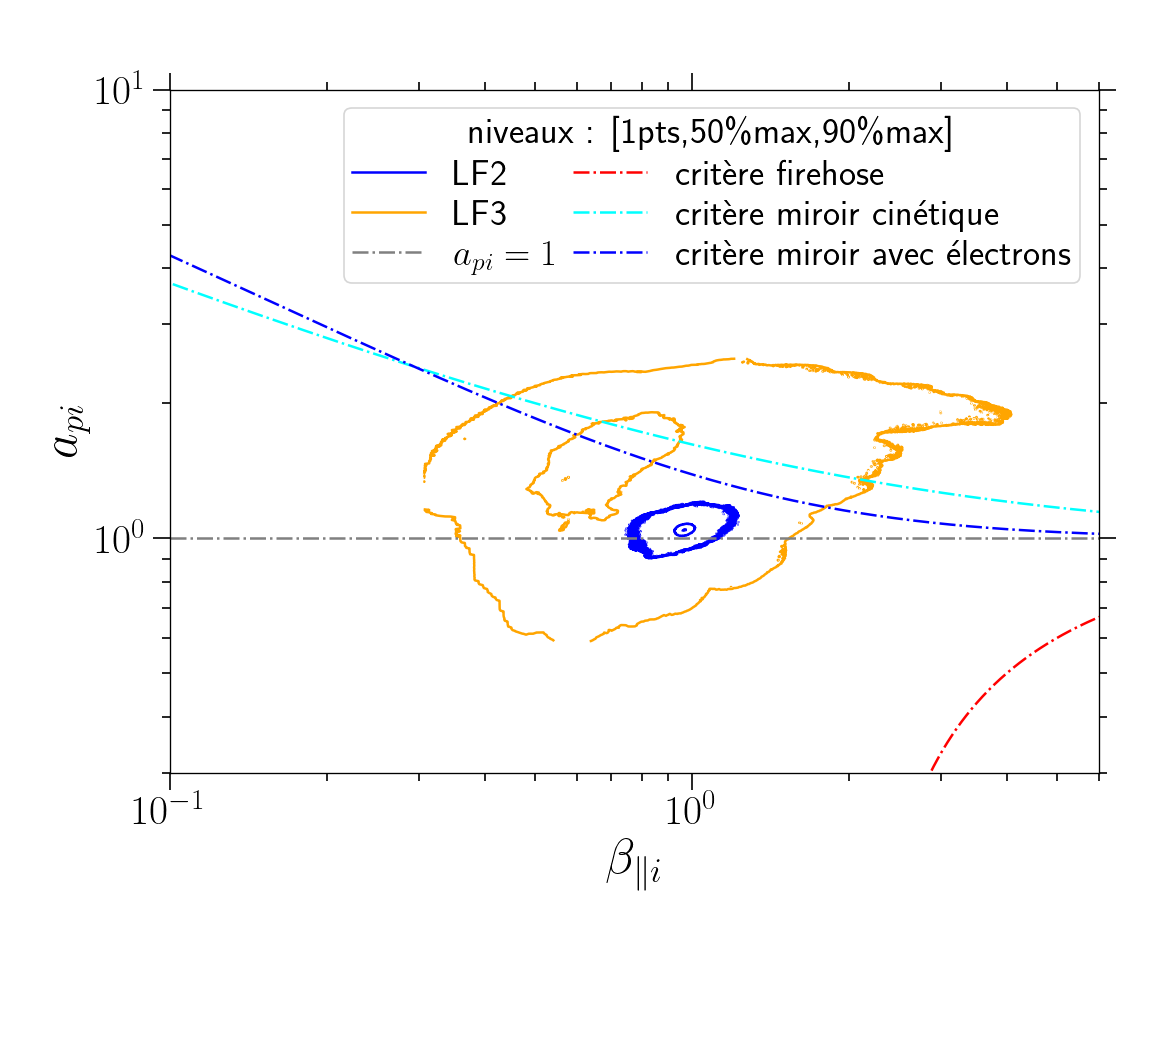
\includegraphics[width=0.9\linewidth,trim=0cm 3cm 1cm 1cm, clip=true]{./Mainmatter/Part_3/images_ch4/diag_simu_LF}
\cprotect\caption{Diagramme \ensuremath{a_{pi}-\beta_{\parallel i}} contenant l'histogramme \cacro{2D} des simulations LF2 et LF3 sous la forme de courbes de niveau centrées sur le couple moyen. Les lignes discontinues correspondent aux critères d'instabilité. Rouge : le critère firehose \cacro{CGL} calculé dans le chapitre \ref{ch-21} et valable dans les modèles cinétique [\cite{hunana_introductory_2019}]. Il ne prend pas en compte l'effet \cacro{Hall}. Cyan : critère miroir cinétique (sans prise en compte de la pression électronique) [\cite{hunana_introductory_2019}]. Bleu : critère miroir proposé par \cite{kuznetsov_mirror_2012}, prenant en compte les électrons gyrotropes et calculé avec $a_{pe} = 1$ et $\beta_{\parallel e } = 1$.}
\label{fig:diag_simu_LF}
\end{figure} 

Les taux d'anisotropie initialisés à $\num{1}$ sont restés proches de 1 et sont moins étalées que ceux des simulations CGL2 et CGL3, même si LF3 montre un étalement plus important que LF2 similairement à CGL3 par rapport à CGL2. Plus d'un tiers de ses points sont situés du côté instable du critère miroir. Deux critères miroirs sont donnés. Le premier en cyan correspond au critère cinétique obtenu en corrigeant le facteur 6 du critère \cacro{CGL} [\cite{galeev_mhd_1983}, \cite{ferriere_mixed_2002}, \cite{hunana_introductory_2019}]. Le second, en bleu, est aussi un critère miroir cinétique mais prenant en compte l'anisotropie de pression électronique. Ce critère est dérivé par \cite{kuznetsov_mirror_2012}. Il est ici représenté en considérant $a_{pe} = 1$ et $\beta_{\parallel e } = 1$. 

Les simulations \cacro{LF} pourraient donc permettre une étude fine de l'impact des instabilités cinétiques sur la cascade turbulente. En première application de la loi exacte étendue, nous avons d'abord cherché à retrouver les résultats de \cite{ferrand_fluid_2021}. 

\section{Premières applications de la loi exacte LF-MHD-Hall-\ensuremath{\nabla P_e}}
\label{sec-343}

Pour les simulations LF2 et LF3, l'extraction d'échantillons de temps consécutifs n'a pas encore été effectuée. On ne fera donc pas apparaître le niveau $\zeta$ dans les résultats préliminaires qui suivent.

\subsection{Effet du flux de chaleur}

L'une des questions que nous nous sommes posées est : retrouve-t-on la décroissance associée au flux de chaleur par \cite{ferrand_fluid_2021} ? On a alors calculé le taux de cascade total $\varepsilon$ dans LF2 et LF3 avec ($\varepsilon|\nabla \cdot \boldsymbol{q} \neq 0$) et sans ($\varepsilon|\nabla \cdot \boldsymbol{q} = 0$) la contribution du flux de chaleur. Les résultats sont montrés sur la \figref{fig:LF_q}.
\begin{figure}[!ht]
 \centering
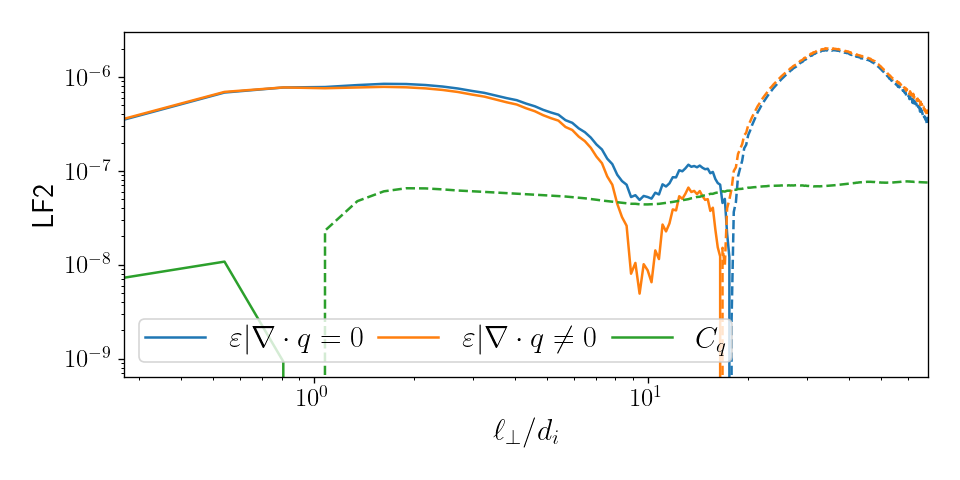
\includegraphics[width=0.9\linewidth,trim=1cm 1cm 0cm 1cm, clip=true]{./Mainmatter/Part_3/images_ch4/LF2_q}
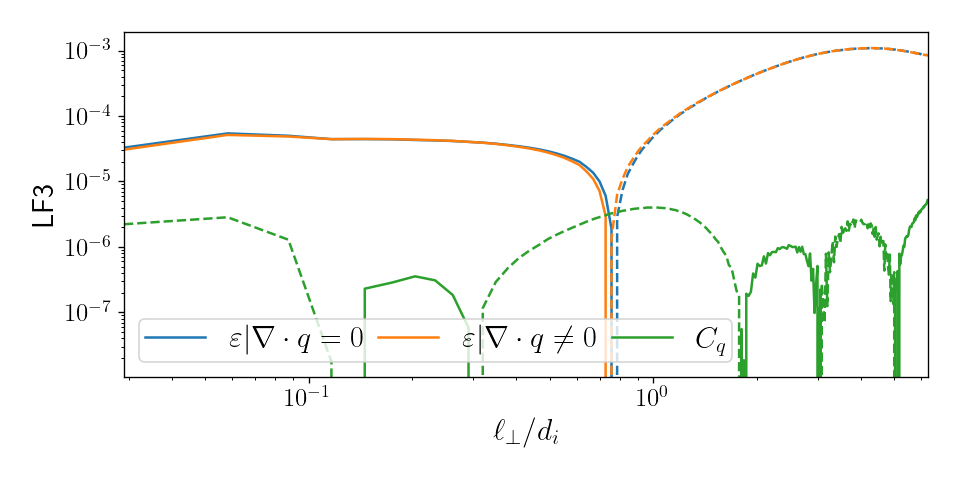
\includegraphics[width=0.9\linewidth,trim=1cm 1cm 0cm 1cm, clip=true]{./Mainmatter/Part_3/images_ch4/LF3_q}
\cprotect\caption{Simu : LF2 (haut) et LF3 (bas). Représentation \cacro{1D} en fonction de \ensuremath{\ell_{\perp}} de la contribution du flux de chaleur \ensuremath{C_q} et du taux de cascade calculé en la prenant en compte (\ensuremath{\varepsilon|\nabla \cdot \boldsymbol{q} \neq 0}) et en l'omettant (\ensuremath{\varepsilon|\nabla \cdot \boldsymbol{q} = 0}).}
\label{fig:LF_q}
\end{figure} 

On remarque que la contribution du flux de chaleur ($C_q$, vert) semble négligeable même aux plus petites échelles. On ne retrouve donc pas la décroissance observée par \cite{ferrand_fluid_2021} en allant vers les petites échelles et que l'on s'attendait à voir pour $\varepsilon|\nabla \cdot \boldsymbol{q} = 0$.

\subsection{Effet des tenseurs de pression}
Afin de vérifier si une erreur ne s'est pas introduite dans notre calcul, nous avons calculé la loi exacte la plus proche de la loi incompressible utilisée par \cite{ferrand_fluid_2021}, c'est-à-dire la loi \cacro{MHDH} en n'y prenant en compte que les contributions isotropes des tenseurs de pression ionique et électronique. En effet, les termes dépendant de l'anisotropie de pression, du terme \cacro{Pe} ou des flux de chaleur sont nouveaux dans l'estimation du taux de cascade. Ce taux de cascade initial, $\varepsilon_{HMHD}$, est représenté en orange sur la \figref{fig:LF_detail}. On retrouve bien le résultat de \cite{ferrand_fluid_2021} avec la décroissance en allant vers les petites échelles. Ayant deux résultats semblant contradictoires, $\varepsilon|\nabla \cdot \boldsymbol{q}$ (bleu) et $\varepsilon_{HMHD}$ (orange), j'ai ajouté une à une les nouvelles contributions afin de comprendre ce qu'il se passait. 

\begin{figure}[!ht]
 \centering
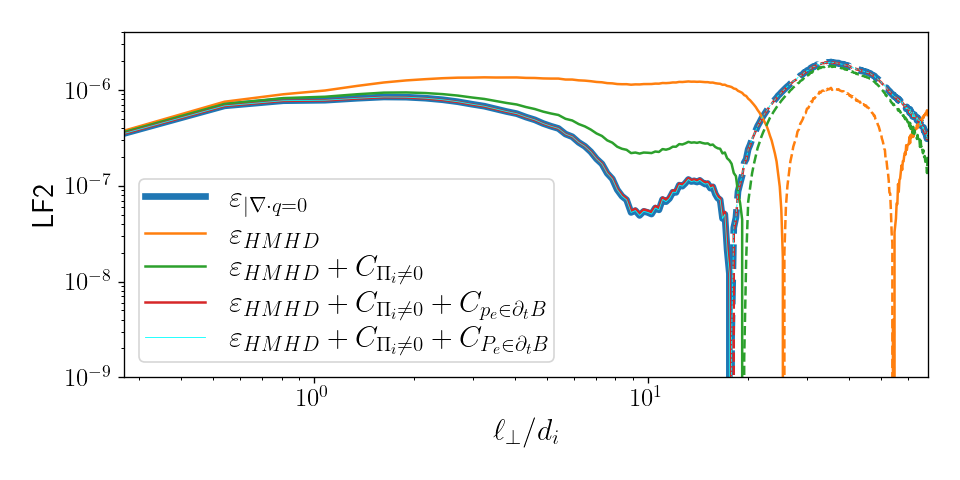
\includegraphics[width=0.9\linewidth,trim=1cm 1cm 0cm 1cm, clip=true]{./Mainmatter/Part_3/images_ch4/LF2_detail}
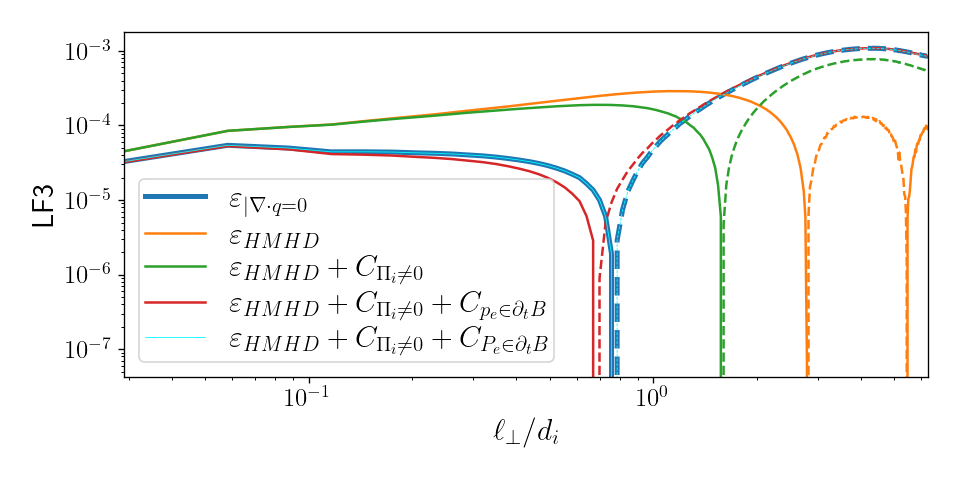
\includegraphics[width=0.9\linewidth,trim=1cm 1cm 0cm 1cm, clip=true]{./Mainmatter/Part_3/images_ch4/LF3_detail}
\cprotect\caption{Simu : LF2 (haut) et LF3 (bas). Représentation \cacro{1D} en fonction de \ensuremath{\ell_{\perp}} du taux de transfert non linéaire \ensuremath{\varepsilon|\nabla \cdot \boldsymbol{q} = 0} (courbe bleue épaisse) calculé en prenant petit à petit en compte les nouvelles contributions. Le but étant de retrouver ce taux de transfert en partant d'une loi \cacro{MHDH} (\ensuremath{\varepsilon_{HMHD}}, orange). Etape 1 (vert) : ajout de l'anisotropie de pression ionique (\ensuremath{C_{\Pi_i \neq 0}}). Etape 2 (rouge) : ajout de la contribution de pression électronique isotrope dans le terme \cacro{Pe} (\ensuremath{C_{p_e \in \partial_t B}}). Etape 3 (cyan) : prise en compte de la contribution complète du tenseur de pression électronique (\ensuremath{C_{P_e \in \partial_t B}}). Le taux de référence est quasiment retrouvé en ajoutant l'anisotropie de pression ionique et la pression isotrope électronique dans le terme \cacro{Pe}.}
\label{fig:LF_detail}
\end{figure} 

 Tout d'abord, on prend en compte l'anisotropie de pression des ions et des électrons en gardant une loi d'Ohm \cacro{MHDH}. Le résultat correspond à la courbe verte. Le niveau du taux de cascade commence à s'affaisser aux échelles a priori inertielles, et à augmenter près des échelles de forçage. Ces ajouts sont dominés par la pression ionique.

Ensuite, on ajoute la contribution de la pression électronique isotrope associée au terme \cacro{Pe} de la loi d'Ohm, cela donne la courbe rouge. Le résultat est alors très proche du résultat voulu. La contribution de la composante anisotrope des tenseurs de pression électronique dans ce terme (résultat cyan) s'avère faible pour LF2 et influe un peu plus sur le taux de transfert de LF3. Le résultat  $\varepsilon|\nabla \cdot \boldsymbol{q}$ observé sur la \figref{fig:LF_q} est ainsi retrouvé.

Ce résultat semble paradoxal face aux conclusions de \cacro{F21}. Dans cet article, ils concluent en comblant la décroissance du taux de cascade par une estimation d'un taux de dissipation dû à l'amortissement Landau, remontant ainsi le niveau du taux de cascade dans la zone inertielle. De notre côté, on observe plutôt un affaissement du niveau du taux de cascade dû à la prise en compte de l'anisotropie de pression ionique ainsi que du tenseur de pression électronique dans l'équation d'induction. {\bf Ces résultats obtenus très récemment semblent venir questionner ou la méthode d'obtention du taux de dissipation par effet Landau utilisée par \cite{ferrand_fluid_2021}, ou notre interprétation de la contribution du flux de chaleur dans le taux de cascade. Leur compréhension demande une analyse plus fine que ce qui a pu être fait jusqu'à présent.} 

